\documentclass[12pt, twoside]{article}
\usepackage[letterpaper, margin=1in, headsep=0.5in]{geometry}
\usepackage[english]{babel}
\usepackage[utf8]{inputenc}
\usepackage{amsmath}
\usepackage{amsfonts}
\usepackage{amssymb}
\usepackage{tikz}
\usetikzlibrary{quotes, angles}
\usepackage{graphicx}
\usepackage{enumitem}
\usepackage{multicol}
\usepackage{hyperref}

\newif\ifmeta
\metatrue %print standards and topics tags

\title{IB Mathematics}
\author{Chris Huson}
\date{March 2022}

\usepackage{fancyhdr}
\pagestyle{fancy}
\fancyhf{}
\renewcommand{\headrulewidth}{0pt} % disable the underline of the header
\raggedbottom


\fancyhead[LE]{\thepage}
\fancyhead[RO]{\thepage \\ Name: \hspace{4cm} \,\\}
\fancyhead[LO]{BECA / IB Math 5 Exponential functions \\* 3 March 2022}

\begin{document}
\subsubsection*{5.7 Classwork: The natural base \emph{e}}
I can calculate continuous compounding \hfill CCSS.HSF.LE.A.2 \\[0.5cm]
$\displaystyle FV=PV \times \left(1+\frac{r}{100k} \right)^{kn}$
where FV is the future value,\\[0.25cm]
PV is the present value, n is the number of years, \\
 k is the number of compounding periods per year, \\
 r\% is the nominal annual rate of interest

\begin{enumerate}
\item Do Now: A seven year investment of \$100,000 earns an annual interest rate of 8.25\%.
\begin{enumerate}[itemsep=2cm]
    \item Find the future value at maturity (after 7 years) with annual compounding. 
    \item Find the value at maturity with monthly compounding.
\end{enumerate} \vspace{2cm}

\item On the grid below draw the exponential function $\displaystyle f(t)=1700 \times \left( 1+0.095 \right)^t$ representing the growth of an investment over $t$ years.
\begin{multicols}{2}
    \begin{enumerate}[itemsep=1.2cm]
        \item Write down the initial value of the investment.
        \item Write down the annual interest rate.
        \item Find the value of the investment after ten years.\vspace{1cm}
        \item Find the number of years it takes the investment to double in value.
    \end{enumerate}
    \begin{center}
    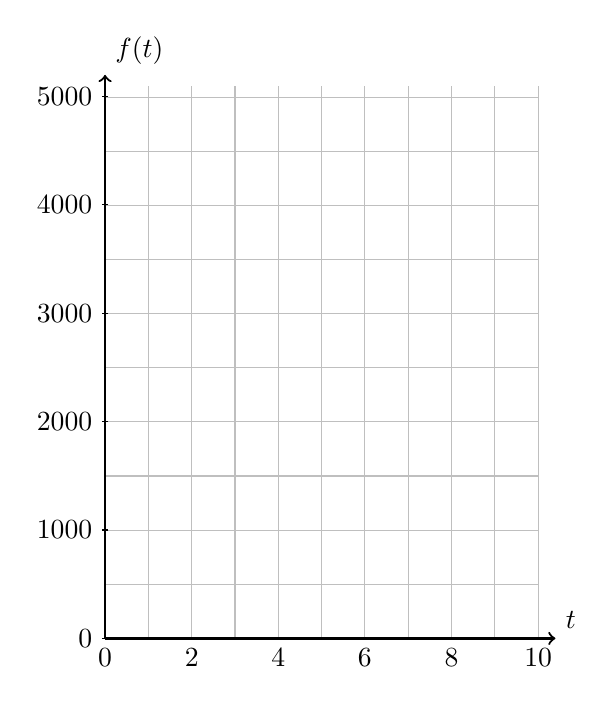
\begin{tikzpicture}[x=1cm, y=0.0025cm, scale=0.55]
        \draw [thin, color=lightgray,xstep=1.0cm,ystep=1.25cm](0,0) grid (10,5100);
        \draw [thick, ->] (0,0) -- (+10.4,0) node [above right]{$t$};
        \draw [thick, ->] (0,0) -- (0,5200) node [above right]{$f(t)$};        
        \foreach \x in {0,2,...,10}
            \draw (\x cm,0) -- (\x cm,0) node[below] {$\x$};
        \foreach \y in {0,1000,...,5000}
            \draw[shift={(0,\y)}] (2pt,0pt)--(-2pt,0pt) node[left]{$\y$};
        %\draw [thick, smooth,domain=0:10] plot(\x,{1700*(1.095^\x)});
    \end{tikzpicture}
    \end{center}
    \end{multicols}

\newpage
\subsubsection*{The natural base $e \approx 2.71828 ...$}
\item Find each value using a calculator or computer
\begin{multicols}{2}
    \begin{enumerate}
        \item $e^{0.10}=$
        \item $e^{2}=$
    \end{enumerate}
\end{multicols}

\item The temperature of a hot iron as it cools is modeled by the function 
    \[ T(x)=350e^{-0.035x}+18 \] where $T(x)$
    is the temperature in degrees Celsius and $x$ is the time in minutes.
    \begin{enumerate}[itemsep=1cm]
        \item Write down the initial temperature at time zero.
        \item Find the temperature after 20 minutes.
        \item When will the temperature of the iron reach 75 degrees Celsius?
        \item On the graph below, sketch the temperature of the iron, labeling the points above A, B, and C.
    \end{enumerate}
    \begin{center}
    \begin{tikzpicture}[xscale= 0.2, yscale=0.015]
        \draw [thick, ->] (0,0) -- (62,0) node [right] {$x$};
        \draw [thick, ->] (0,0) -- (0,550) node [right] {$T(x)$};
        \foreach \x in {0,10,20,30,40,50,60}
            \draw[shift={(\x,0)}] (0,10) -- (0,0) node[below]  {$\x$};
        \foreach \y in {0,100,200,300,400,500}
            \draw[shift={(0,\y)}] (0.5,0) -- (0,0) node[left]  {$\y$};
        %\draw [<-, ->] plot[domain= 0:60] (\x,{350*exp(-0.035*\x) +18});
        %\draw plot[domain=0:60] (\x, 75);
    \end{tikzpicture}
    \end{center}

\end{enumerate}
\end{document}
